\documentclass[aspectratio=169,10pt]{beamer}
\usetheme{Madrid}
\usecolortheme{default}
\usepackage{fontspec}
\setmainfont{Times New Roman}
\setsansfont{Arial}
\usepackage{booktabs}
\usepackage{graphicx}
\usepackage{array}
\graphicspath{{../figures/}}
\setbeamertemplate{navigation symbols}{}
\setbeamertemplate{caption}[numbered]
\setbeamertemplate{itemize items}[circle]
\definecolor{FreshGreen}{RGB}{31,121,74}
\setbeamercolor{structure}{fg=FreshGreen}
\setbeamercolor{frametitle}{fg=white,bg=FreshGreen}
\setbeamercolor{title}{fg=white,bg=FreshGreen}

\title[FreshRetailNet-50K]{Dự báo nhu cầu bán lẻ có xét stockout}
\subtitle{Two-stage latent demand recovery + daily forecasting trên FreshRetailNet-50K}
\author{}
\date{}

\begin{document}

\begin{frame}
    \titlepage
\end{frame}

\begin{frame}{Framing vấn đề}
    \begin{block}{Không chỉ là bài toán dự báo sales}
    Observed sales trong bán lẻ có thể bị \textbf{censor} bởi stockout: bán thấp chưa chắc là nhu cầu thấp, mà có thể là không còn hàng để bán.
    \end{block}
    \vspace{0.15cm}
    \begin{columns}[T]
        \begin{column}{0.49\linewidth}
            \textbf{Nếu forecast trực tiếp observed sales}
            \begin{itemize}
                \item Model học cả nhu cầu thật lẫn giới hạn tồn kho.
                \item Dễ under-forecast ở nhóm hay hết hàng.
                \item Sai với mục tiêu vận hành: cần dự báo demand để chuẩn bị hàng.
            \end{itemize}
        \end{column}
        \begin{column}{0.49\linewidth}
            \textbf{Hướng của đồ án}
            \begin{itemize}
                \item Recover latent demand ở giờ stockout.
                \item Aggregate hourly recovered demand lên daily.
                \item Forecast tổng nhu cầu 7 ngày tiếp theo.
            \end{itemize}
        \end{column}
    \end{columns}
\end{frame}

\begin{frame}{Câu hỏi nghiên cứu}
    \begin{enumerate}
        \item Có thể khôi phục demand bị ẩn trong các giờ stockout mà không leakage theo thời gian không?
        \item Imputation có làm tổng demand tăng quá mức hay không?
        \item Forecast trên recovered demand có tốt hơn forecast trên observed sales không?
    \end{enumerate}
    \vspace{0.25cm}
    \begin{block}{Metric chính}
    WAPE = $\sum |y-\hat{y}| / \sum |y|$. Với bài toán này, WAPE cho biết tổng sai số tuyệt đối chiếm bao nhiêu phần trăm tổng nhu cầu thật.
    \end{block}
\end{frame}

\begin{frame}{Contribution của đồ án}
    \begin{columns}[T]
        \begin{column}{0.50\linewidth}
            \textbf{Đóng góp kỹ thuật}
            \begin{itemize}
                \item Framing lại bài toán từ observed sales sang recovered demand.
                \item Hourly stockout recovery theo expanding window, tránh leakage.
                \item Calibration + cap q90 + sensitivity để kiểm soát imputation.
            \end{itemize}
        \end{column}
        \begin{column}{0.48\linewidth}
            \textbf{Đóng góp business}
            \begin{itemize}
                \item Ước lượng phần demand bị che bởi stockout.
                \item Chỉ ra weekly seasonality là baseline vận hành rất mạnh.
                \item Đề xuất hybrid seasonal-ML cho replenishment forecast.
            \end{itemize}
        \end{column}
    \end{columns}
    \vspace{0.2cm}
    \begin{block}{Không overclaim}
    Đồ án không claim recovered demand là ground truth tuyệt đối; đây là proxy được kiểm soát và kiểm tra bằng validation/sensitivity.
    \end{block}
\end{frame}

\begin{frame}{Dữ liệu và thách thức}
    \begin{columns}[T]
        \begin{column}{0.48\linewidth}
            \begin{tabular}{lr}
                \toprule
                Mẫu sử dụng & 0.1 \\
                Số quan sát hourly & 11640000 \\
                Số chuỗi & 5000 \\
                Bắt đầu & 2024-03-28 00:00:00 \\
                Kết thúc & 2024-07-02 23:00:00 \\
                Stockout row rate & 24.65\% \\
                \bottomrule
            \end{tabular}
            \vspace{0.25cm}
            \begin{itemize}
                \item Nhiều chuỗi store--product.
                \item Demand thưa, nhiều zero và spike.
                \item Có promotion, weather, calendar và stockout.
            \end{itemize}
        \end{column}
        \begin{column}{0.50\linewidth}
            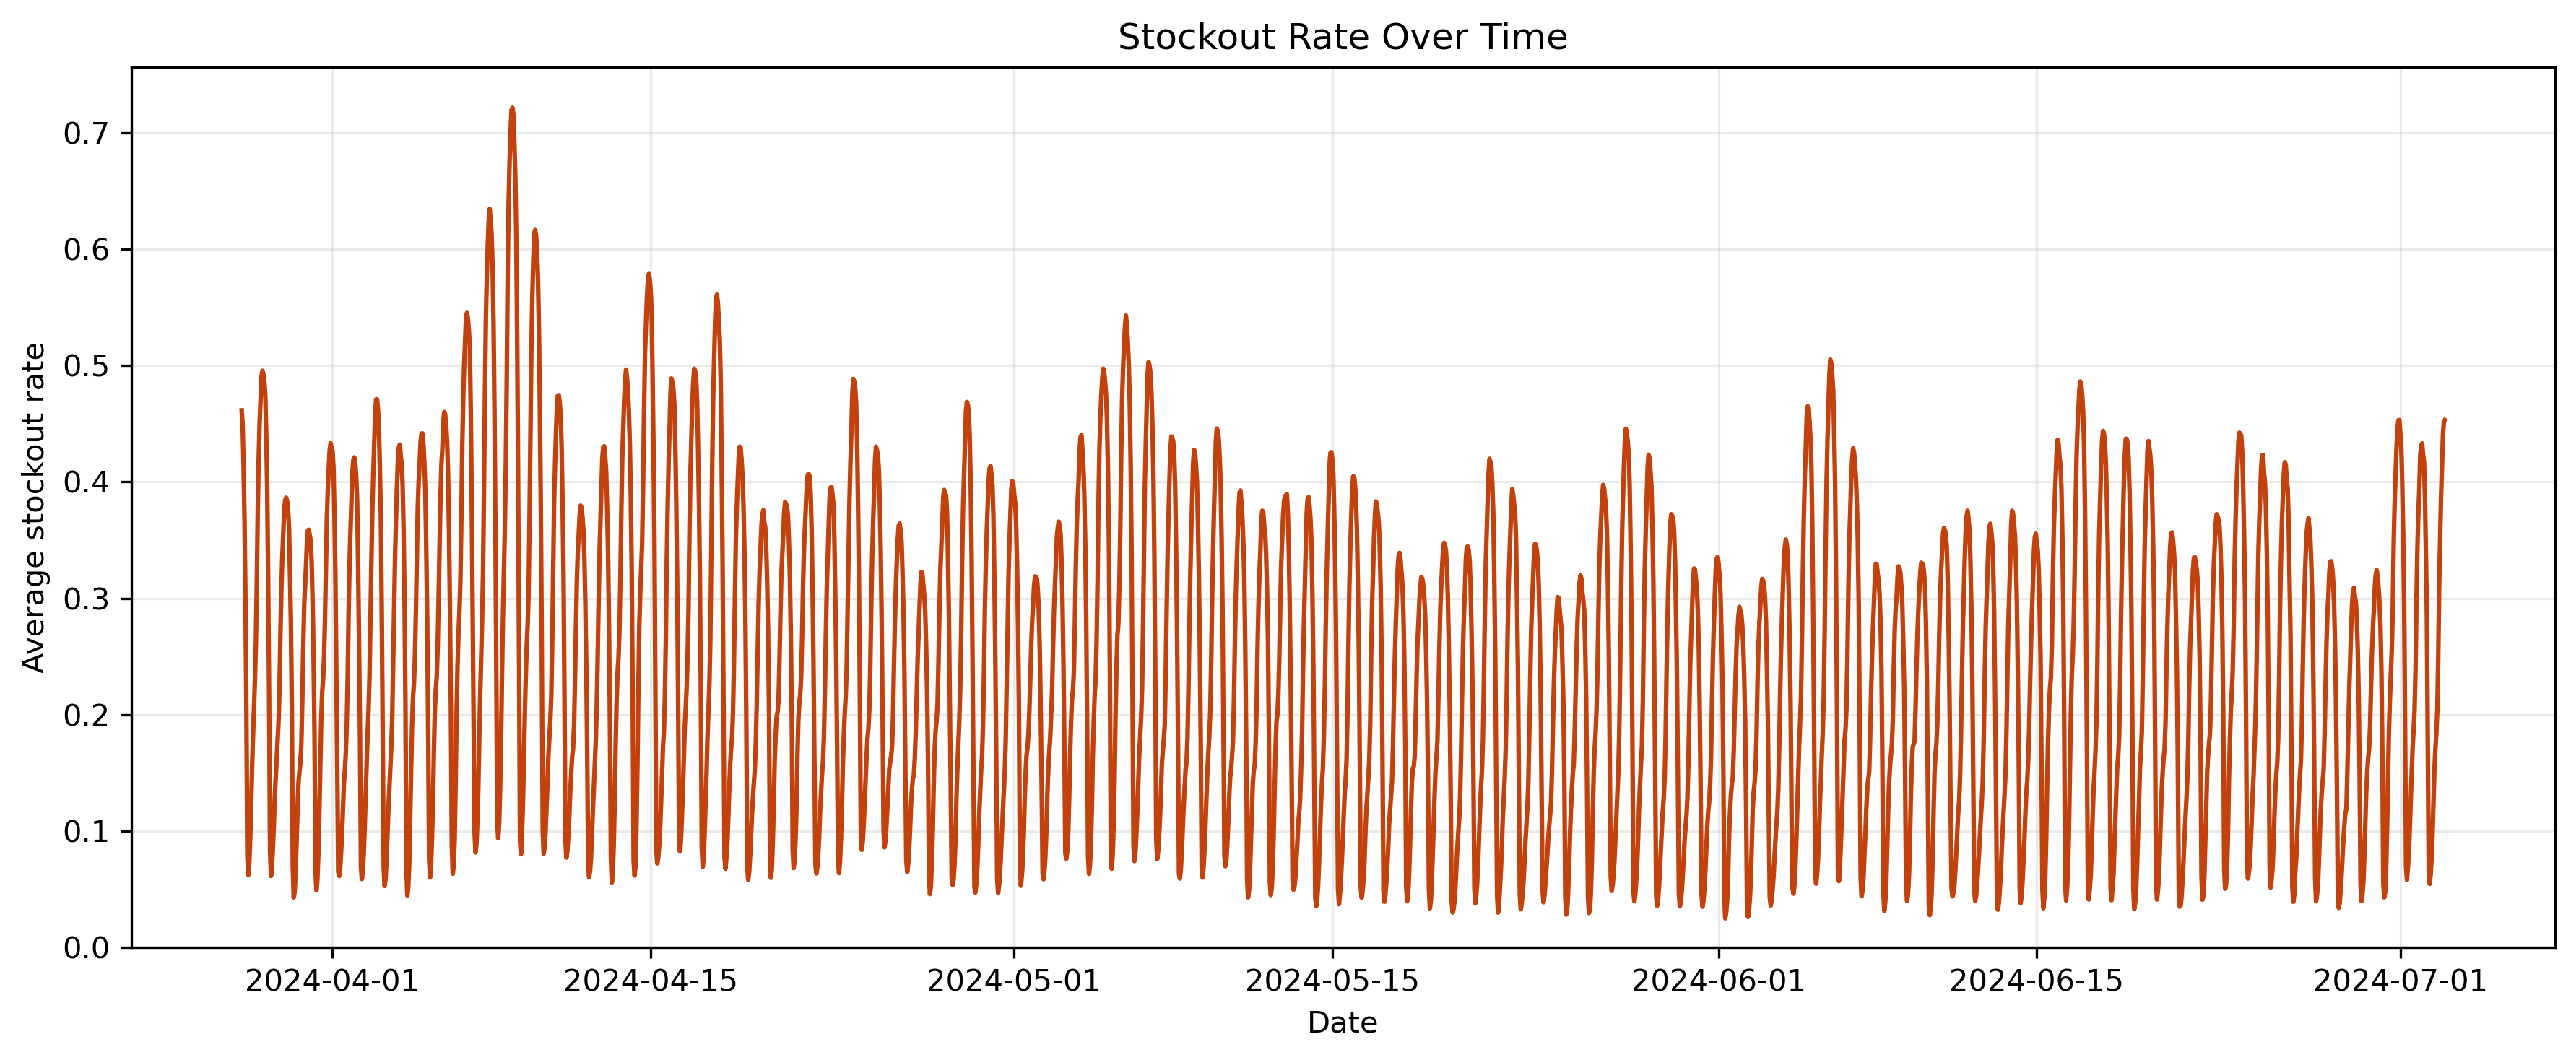
\includegraphics[width=\linewidth]{stockout_rate_over_time.png}
        \end{column}
    \end{columns}
\end{frame}

\begin{frame}{Vì sao không dùng mô hình cổ điển làm chính?}
    \begin{columns}[T]
        \begin{column}{0.5\linewidth}
            \textbf{ARIMA/SARIMA riêng từng chuỗi}
            \begin{itemize}
                \item Khó scale cho nhiều store--product.
                \item Không ổn với chuỗi thưa và nhiều zero.
                \item Khó đưa đầy đủ promotion, weather, stockout.
            \end{itemize}
        \end{column}
        \begin{column}{0.5\linewidth}
            \textbf{Deep learning}
            \begin{itemize}
                \item Có thể dùng, nhưng tốn tuning và tài nguyên.
                \item Khó bảo vệ nếu dữ liệu/validation chưa thật chặt.
                \item Đồ án ưu tiên pipeline rõ, tái lập, giải thích được.
            \end{itemize}
        \end{column}
    \end{columns}
    \vspace{0.2cm}
    \begin{block}{Lựa chọn chính}
    LightGBM toàn cục: học chung pattern giữa nhiều chuỗi, xử lý phi tuyến tốt, chạy nhẹ, và dễ kết hợp feature engineering.
    \end{block}
\end{frame}

\begin{frame}{Pipeline tổng quát}
    \centering
    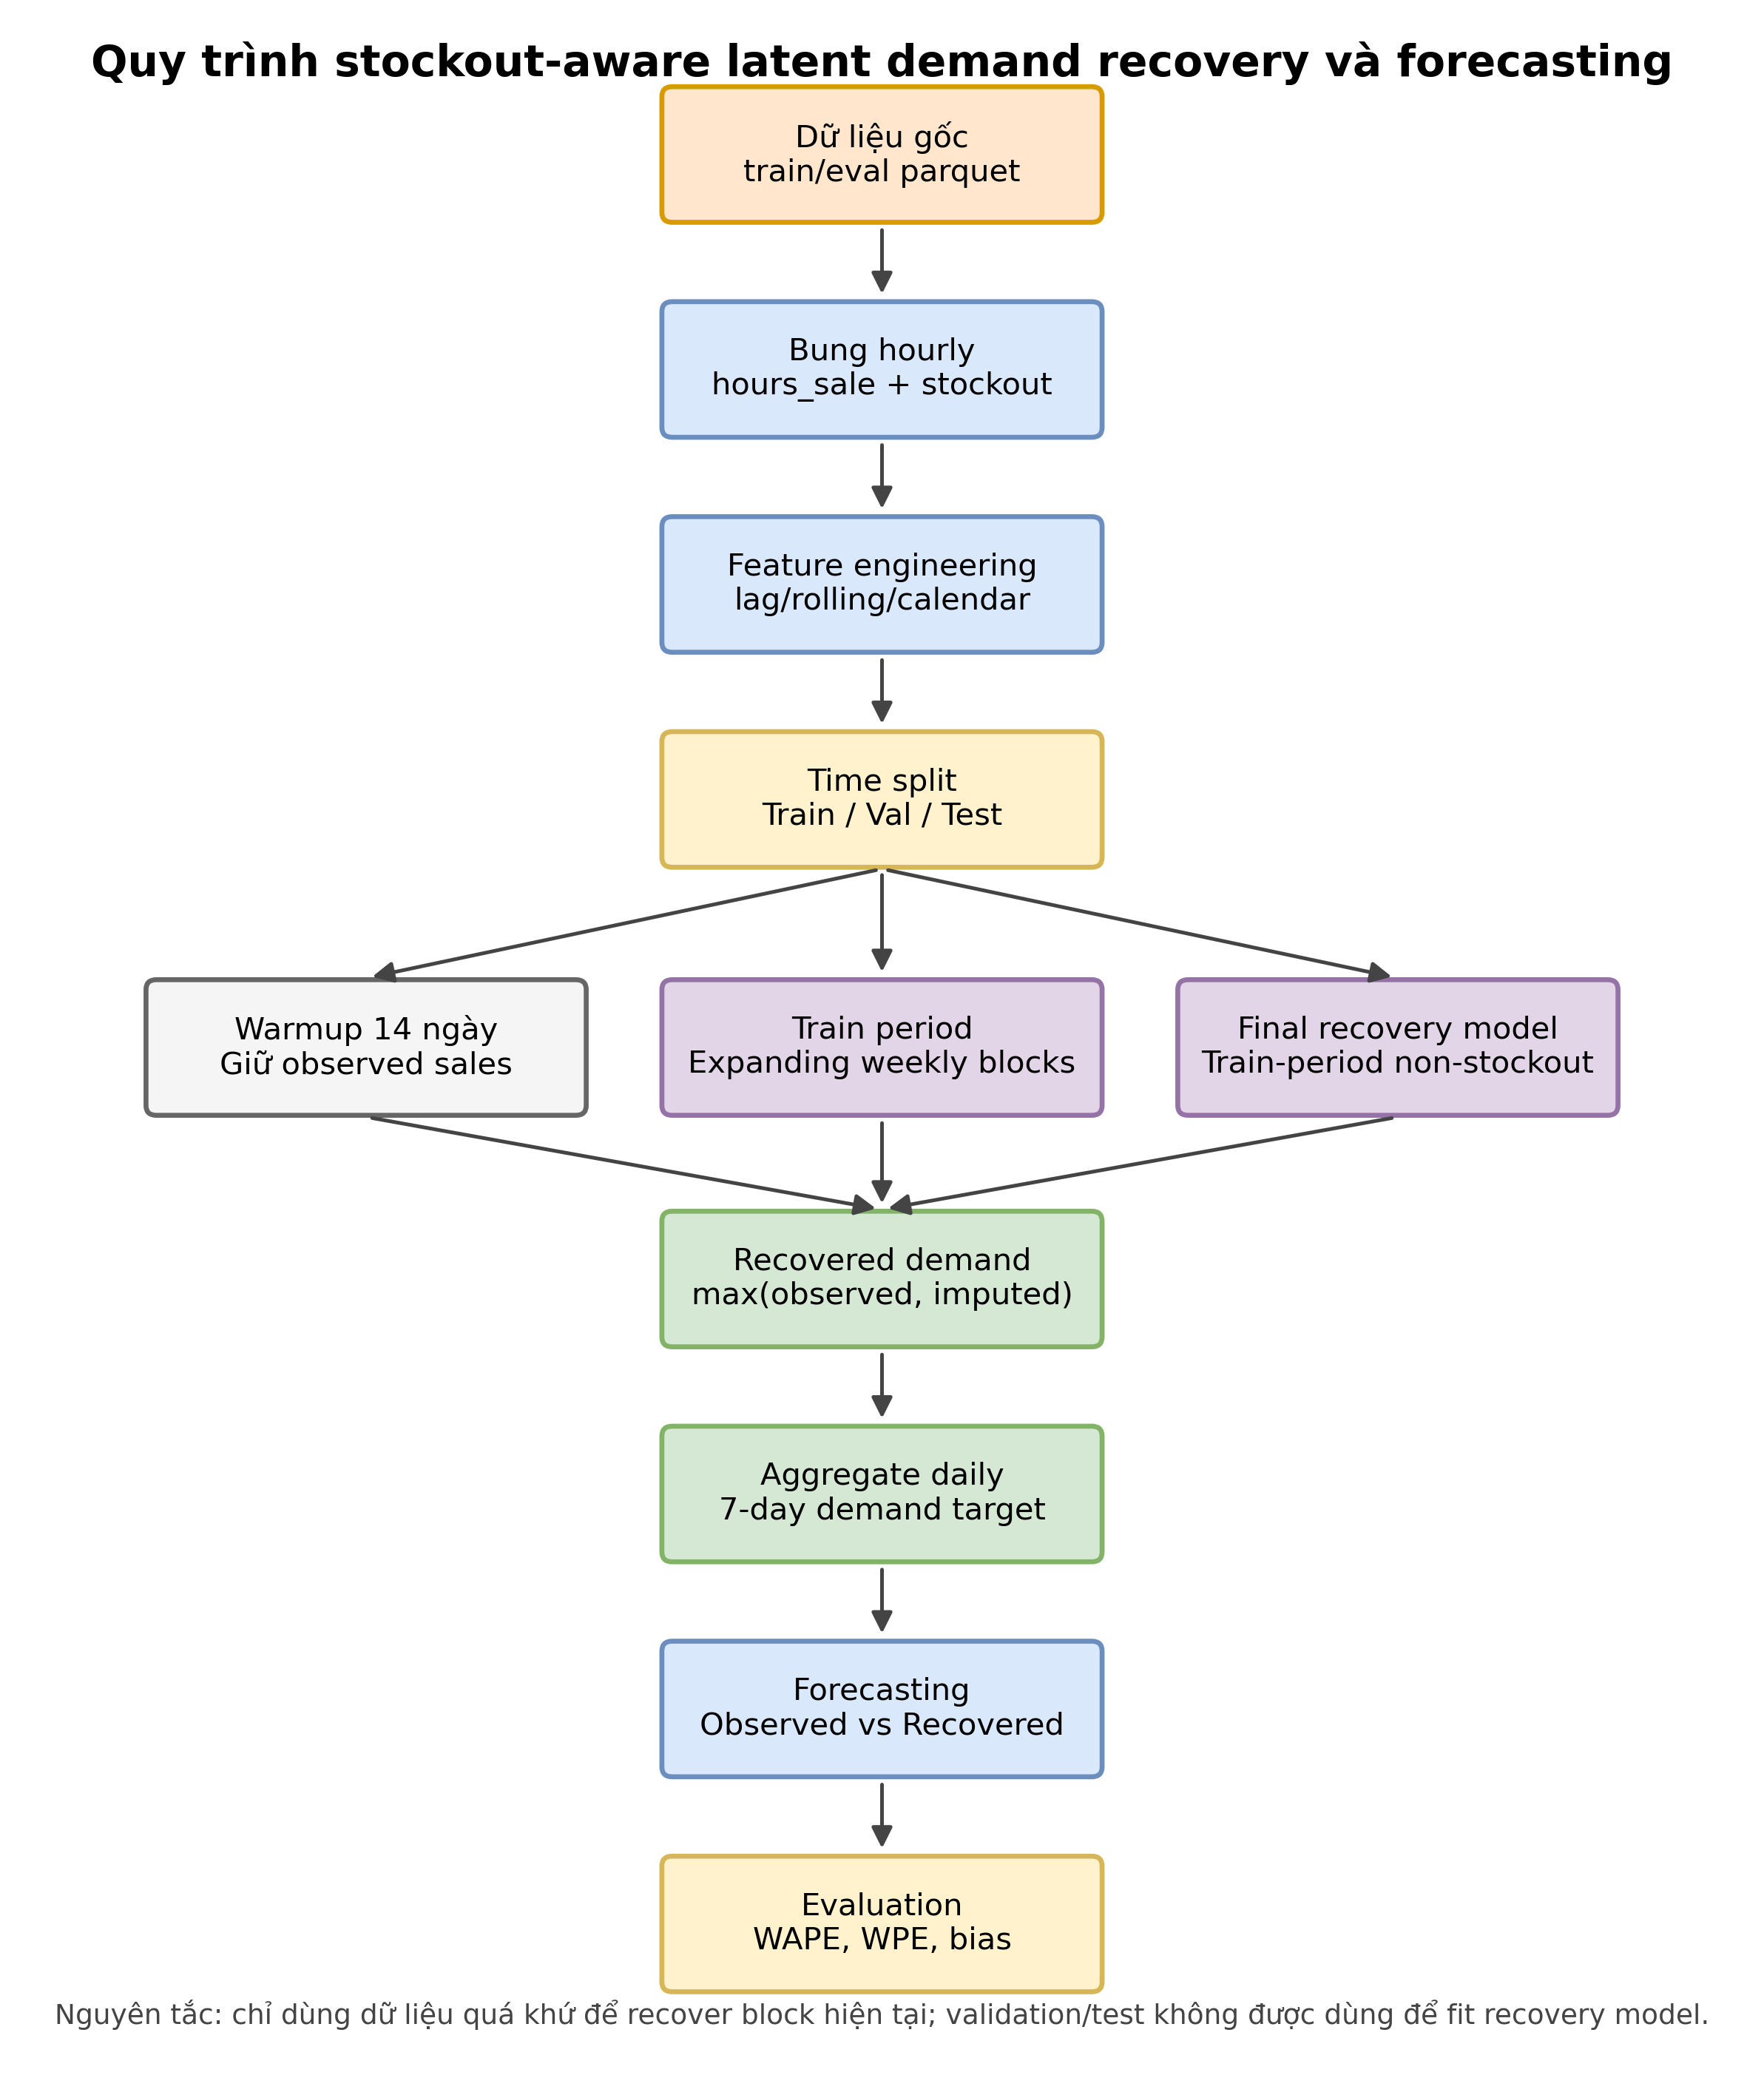
\includegraphics[width=0.92\linewidth,height=0.78\textheight,keepaspectratio]{owner_expanding_window_process.png}
\end{frame}

\begin{frame}{Latent demand recovery không leakage}
    \begin{columns}[T]
        \begin{column}{0.52\linewidth}
            \begin{itemize}
                \item Hourly stockout được recover trước.
                \item Train period dùng expanding window theo block 7 ngày.
                \item Mỗi block chỉ học từ non-stockout rows trong quá khứ.
                \item Warmup 14 ngày để có đủ hai chu kỳ tuần.
                \item Validation/test chỉ dùng model fit từ train-period non-stockout rows.
            \end{itemize}
        \end{column}
        \begin{column}{0.46\linewidth}
            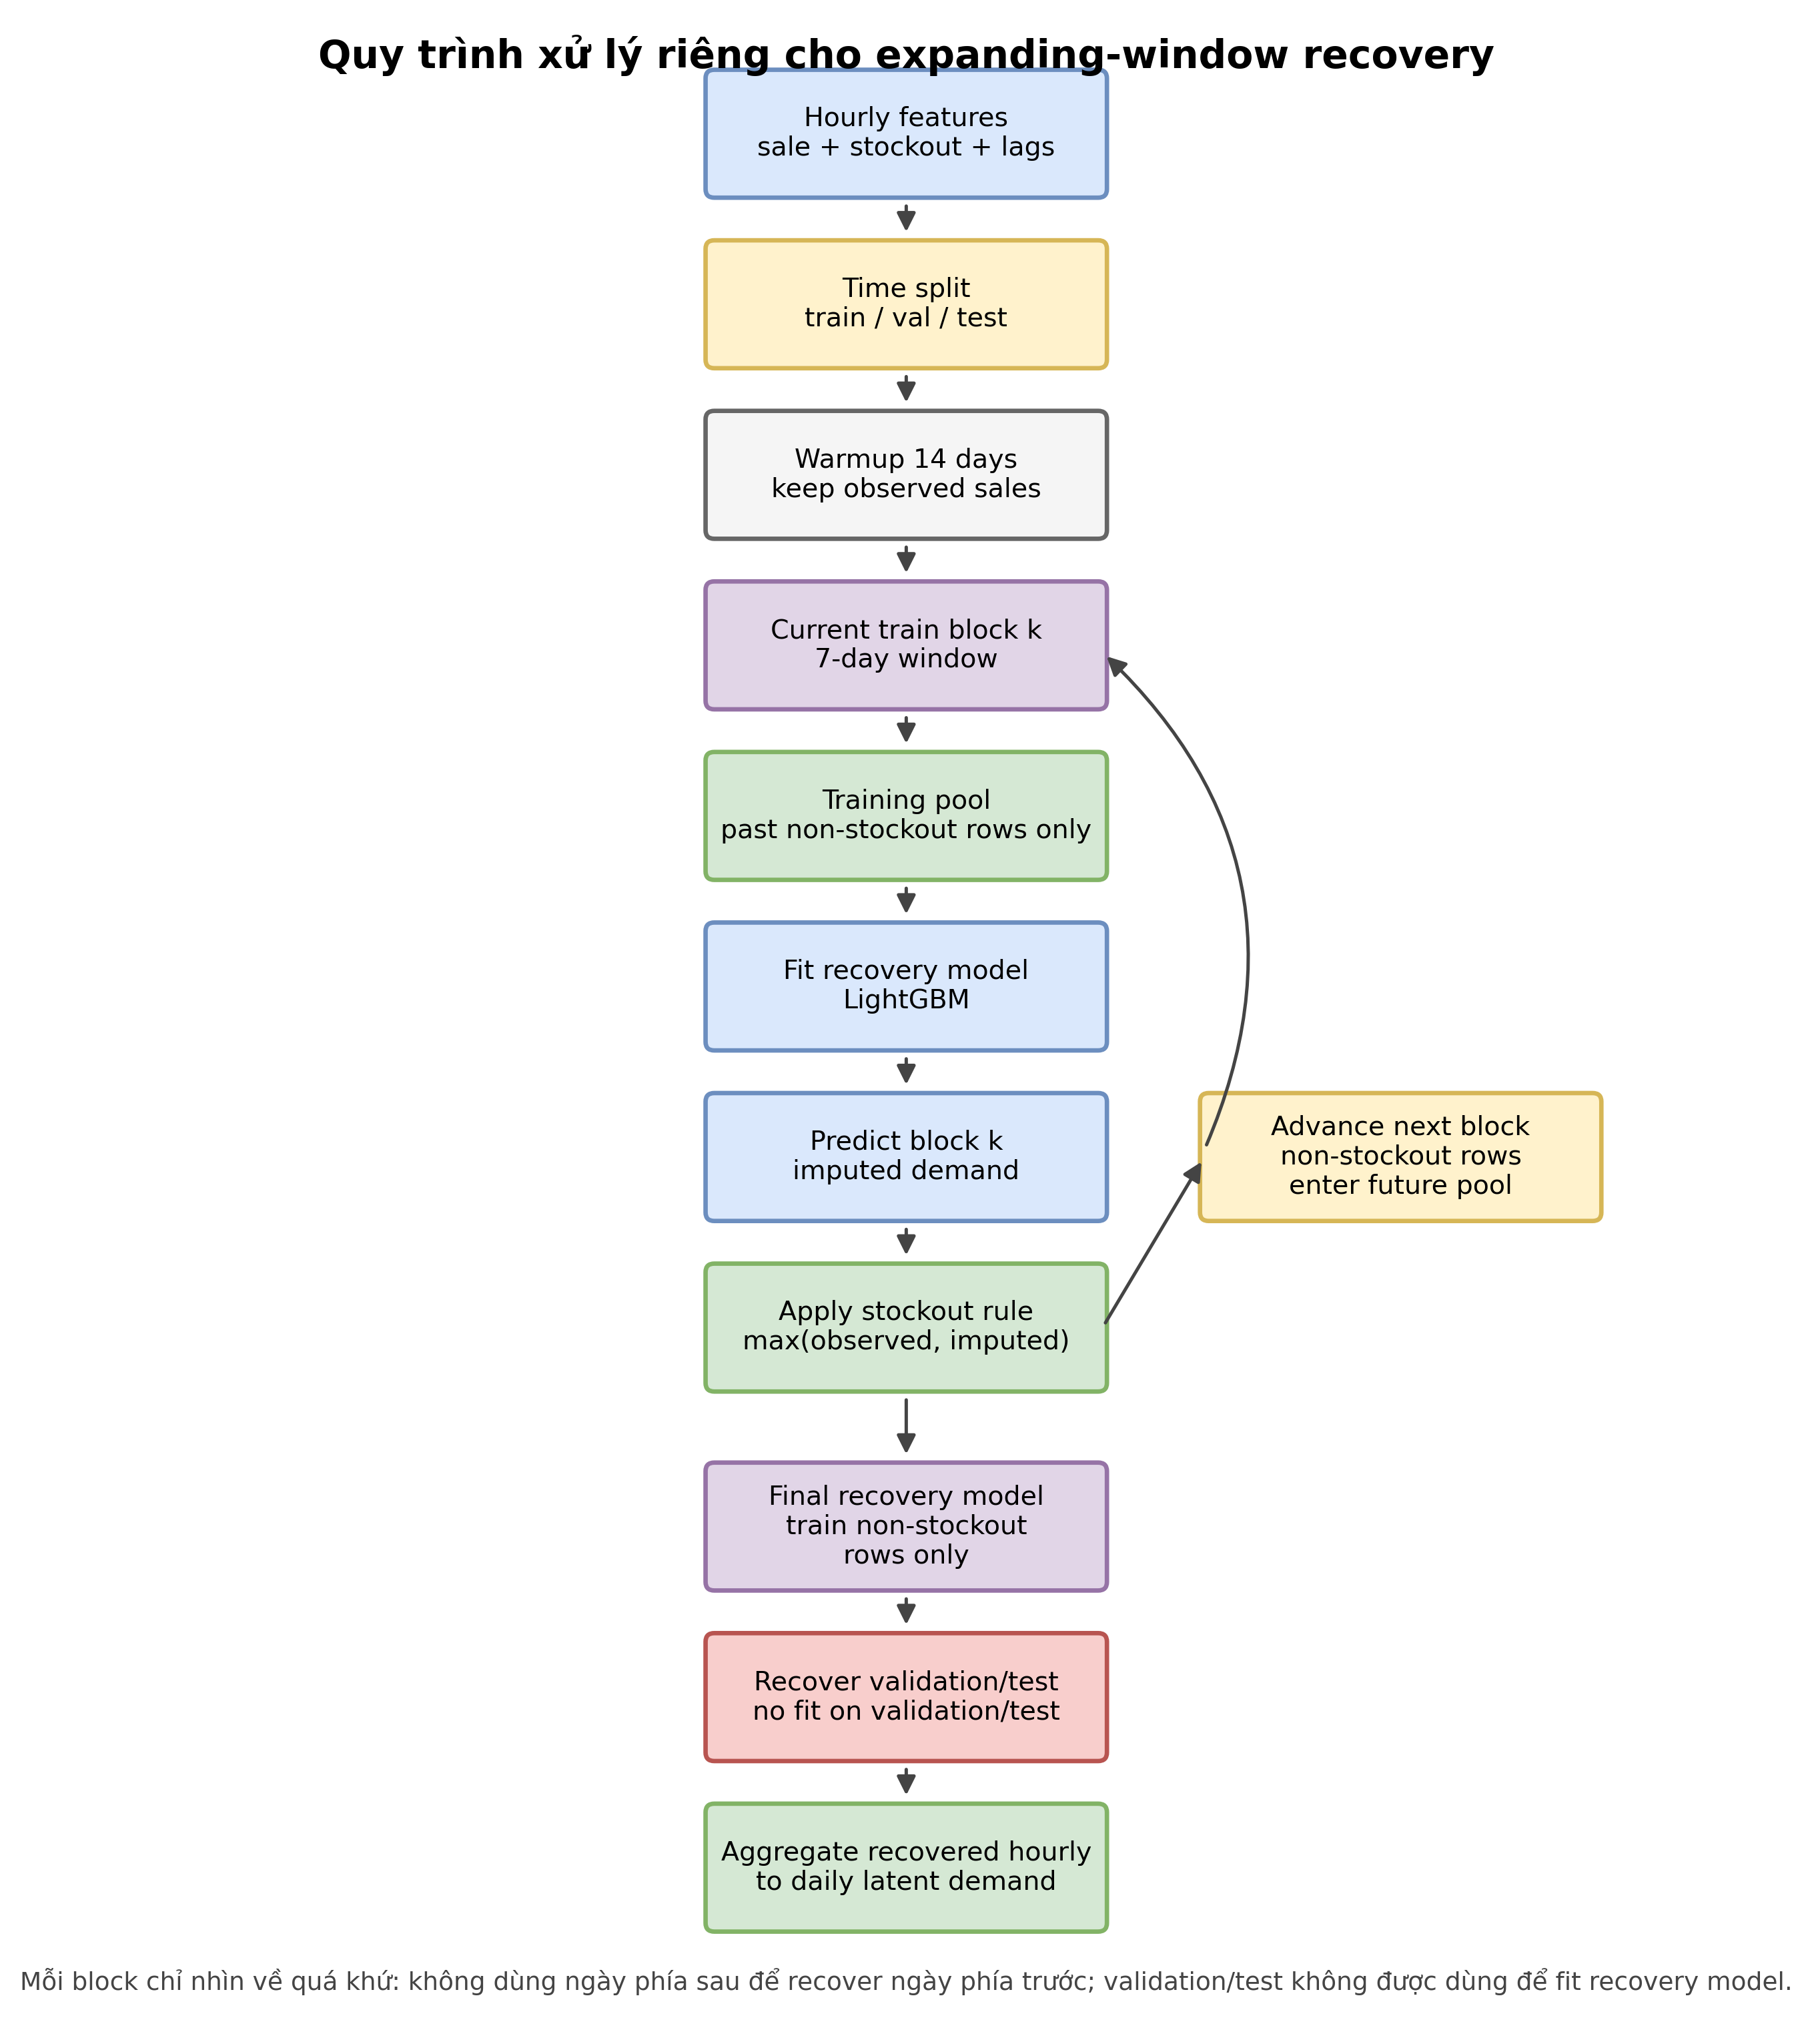
\includegraphics[width=\linewidth,height=0.66\textheight,keepaspectratio]{owner_expanding_window_recovery_detail.png}
        \end{column}
    \end{columns}
\end{frame}

\begin{frame}{Imputation được kiểm soát như thế nào?}
    \begin{block}{Công thức thực tế}
    Raw impute $\rightarrow$ chia calibration factor $\rightarrow$ lấy lost demand dương $\rightarrow$ cap q90 $\rightarrow$ cộng vào observed sales.
    \end{block}
    \begin{columns}[T]
        \begin{column}{0.48\linewidth}
            \begin{tabular}{lr}
                \toprule
                Calibration factor & 1.1298 \\
                Lost demand cap q90 & 0.0663 \\
                Observed sales & 482,697.09 \\
                Recovered demand & 534,270.19 \\
                Recovered lost demand & 51,572.88 \\
                Lift & 10.68\% \\
                \bottomrule
            \end{tabular}
        \end{column}
        \begin{column}{0.48\linewidth}
            \begin{itemize}
                \item Raw calibrated lost demand trước cap: 65,367.58.
                \item Cap q90 giữ lại 78.90\% phần lost demand raw.
                \item Mục tiêu: không để impute quyết định toàn bộ kết quả.
            \end{itemize}
        \end{column}
    \end{columns}
\end{frame}

\begin{frame}{Sensitivity của imputation}
    \begin{columns}[T]
        \begin{column}{0.45\linewidth}
            \begin{tabular}{lrr}
                \toprule
                Kịch bản & Lift & Demand \\
                \midrule
                Cap q75 & 8.51\% & 523,780.62 \\
                Cap q90 & 10.68\% & 534,270.19 \\
                Cap q100 & 13.54\% & 548,064.06 \\
                \bottomrule
            \end{tabular}
            \vspace{0.25cm}
            \begin{itemize}
                \item q90 là lựa chọn cân bằng.
                \item q100 làm lift cao hơn nhưng rủi ro phụ thuộc impute.
            \end{itemize}
        \end{column}
        \begin{column}{0.52\linewidth}
            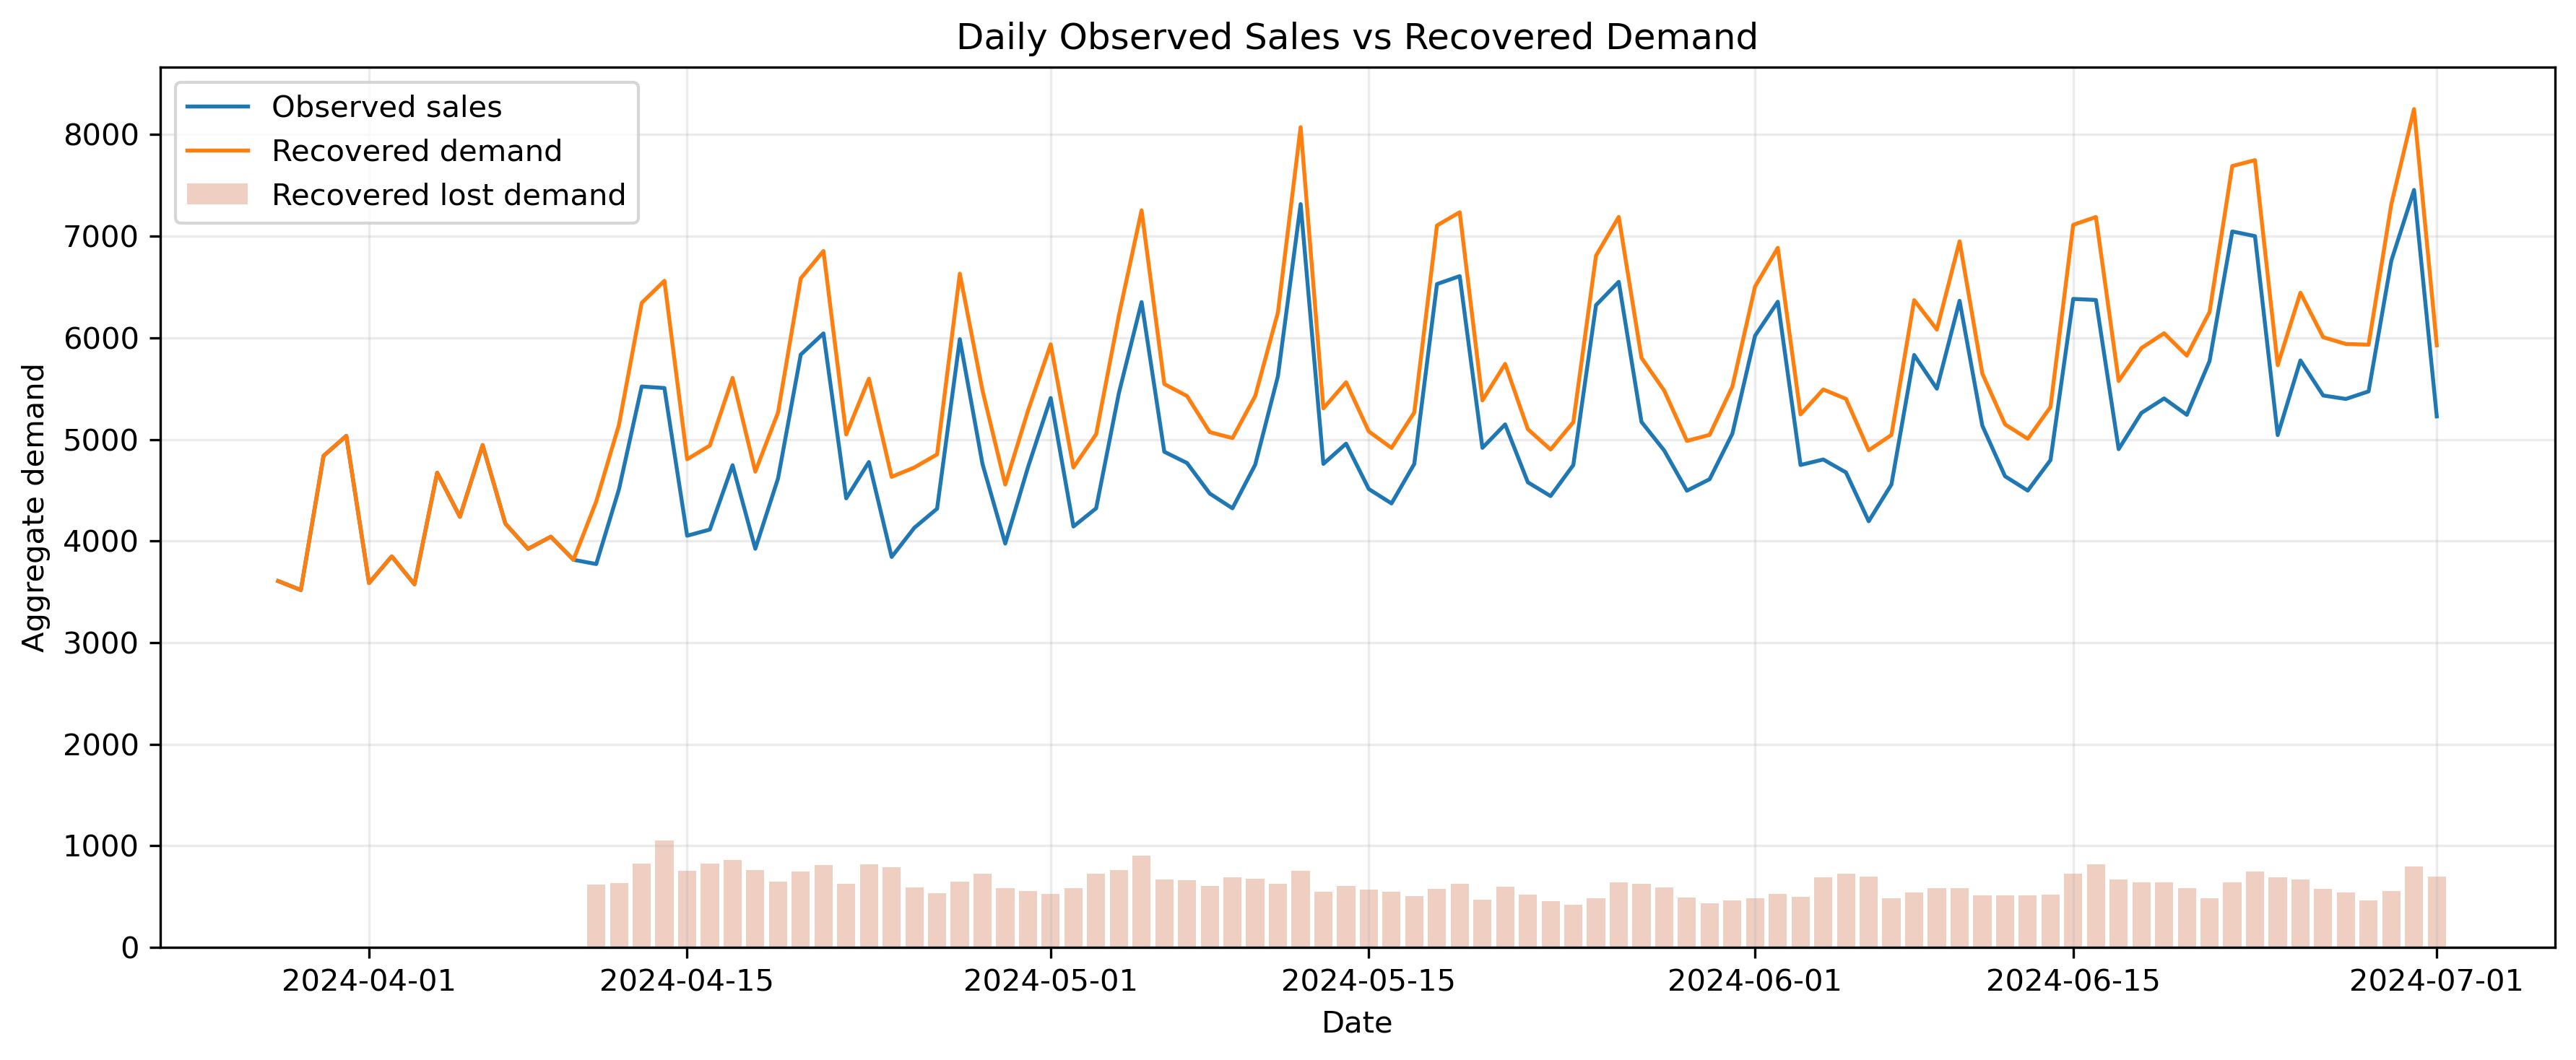
\includegraphics[width=\linewidth]{imputation_daily_uplift.png}
        \end{column}
    \end{columns}
\end{frame}

\begin{frame}{Forecasting setup}
    \begin{columns}[T]
        \begin{column}{0.49\linewidth}
            \textbf{Target chính}
            \begin{itemize}
                \item Hourly recovery.
                \item Aggregate lên daily demand.
                \item Forecast tổng demand 7 ngày tiếp theo.
            \end{itemize}
        \end{column}
        \begin{column}{0.49\linewidth}
            \textbf{So sánh hai hướng}
            \begin{itemize}
                \item Train trên observed sales.
                \item Train trên recovered demand.
                \item Seasonal naive 7 ngày và hybrid seasonal-ML.
                \item Cùng đánh giá trên recovered latent demand proxy.
            \end{itemize}
        \end{column}
    \end{columns}
    \vspace{0.25cm}
    \begin{block}{Baseline phù hợp}
    Seasonal naive là baseline chính vì dữ liệu có chu kỳ tuần rõ; naive/drift/average dùng như đối chứng phụ.
    \end{block}
\end{frame}

\begin{frame}{Kết quả chính}
    \begin{columns}[T]
        \begin{column}{0.48\linewidth}
            \begin{tabular}{lrr}
                \toprule
                Mô hình & WAPE & WPE \\
                \midrule
                Observed-sales & 24.42\% & -17.88\% \\
                Seasonal naive 7-day & 19.85\% & -6.14\% \\
                Recovered LightGBM & 20.28\% & -8.00\% \\
                Seasonal-ML hybrid & 19.67\% & -7.26\% \\
                \bottomrule
            \end{tabular}
            \vspace{0.25cm}
            \begin{itemize}
                \item WAPE giảm tương đối 19.44\% so với observed-sales.
                \item Seasonal naive rất mạnh; hybrid giữ mùa vụ tuần và thêm hiệu chỉnh ML.
            \end{itemize}
        \end{column}
        \begin{column}{0.50\linewidth}
            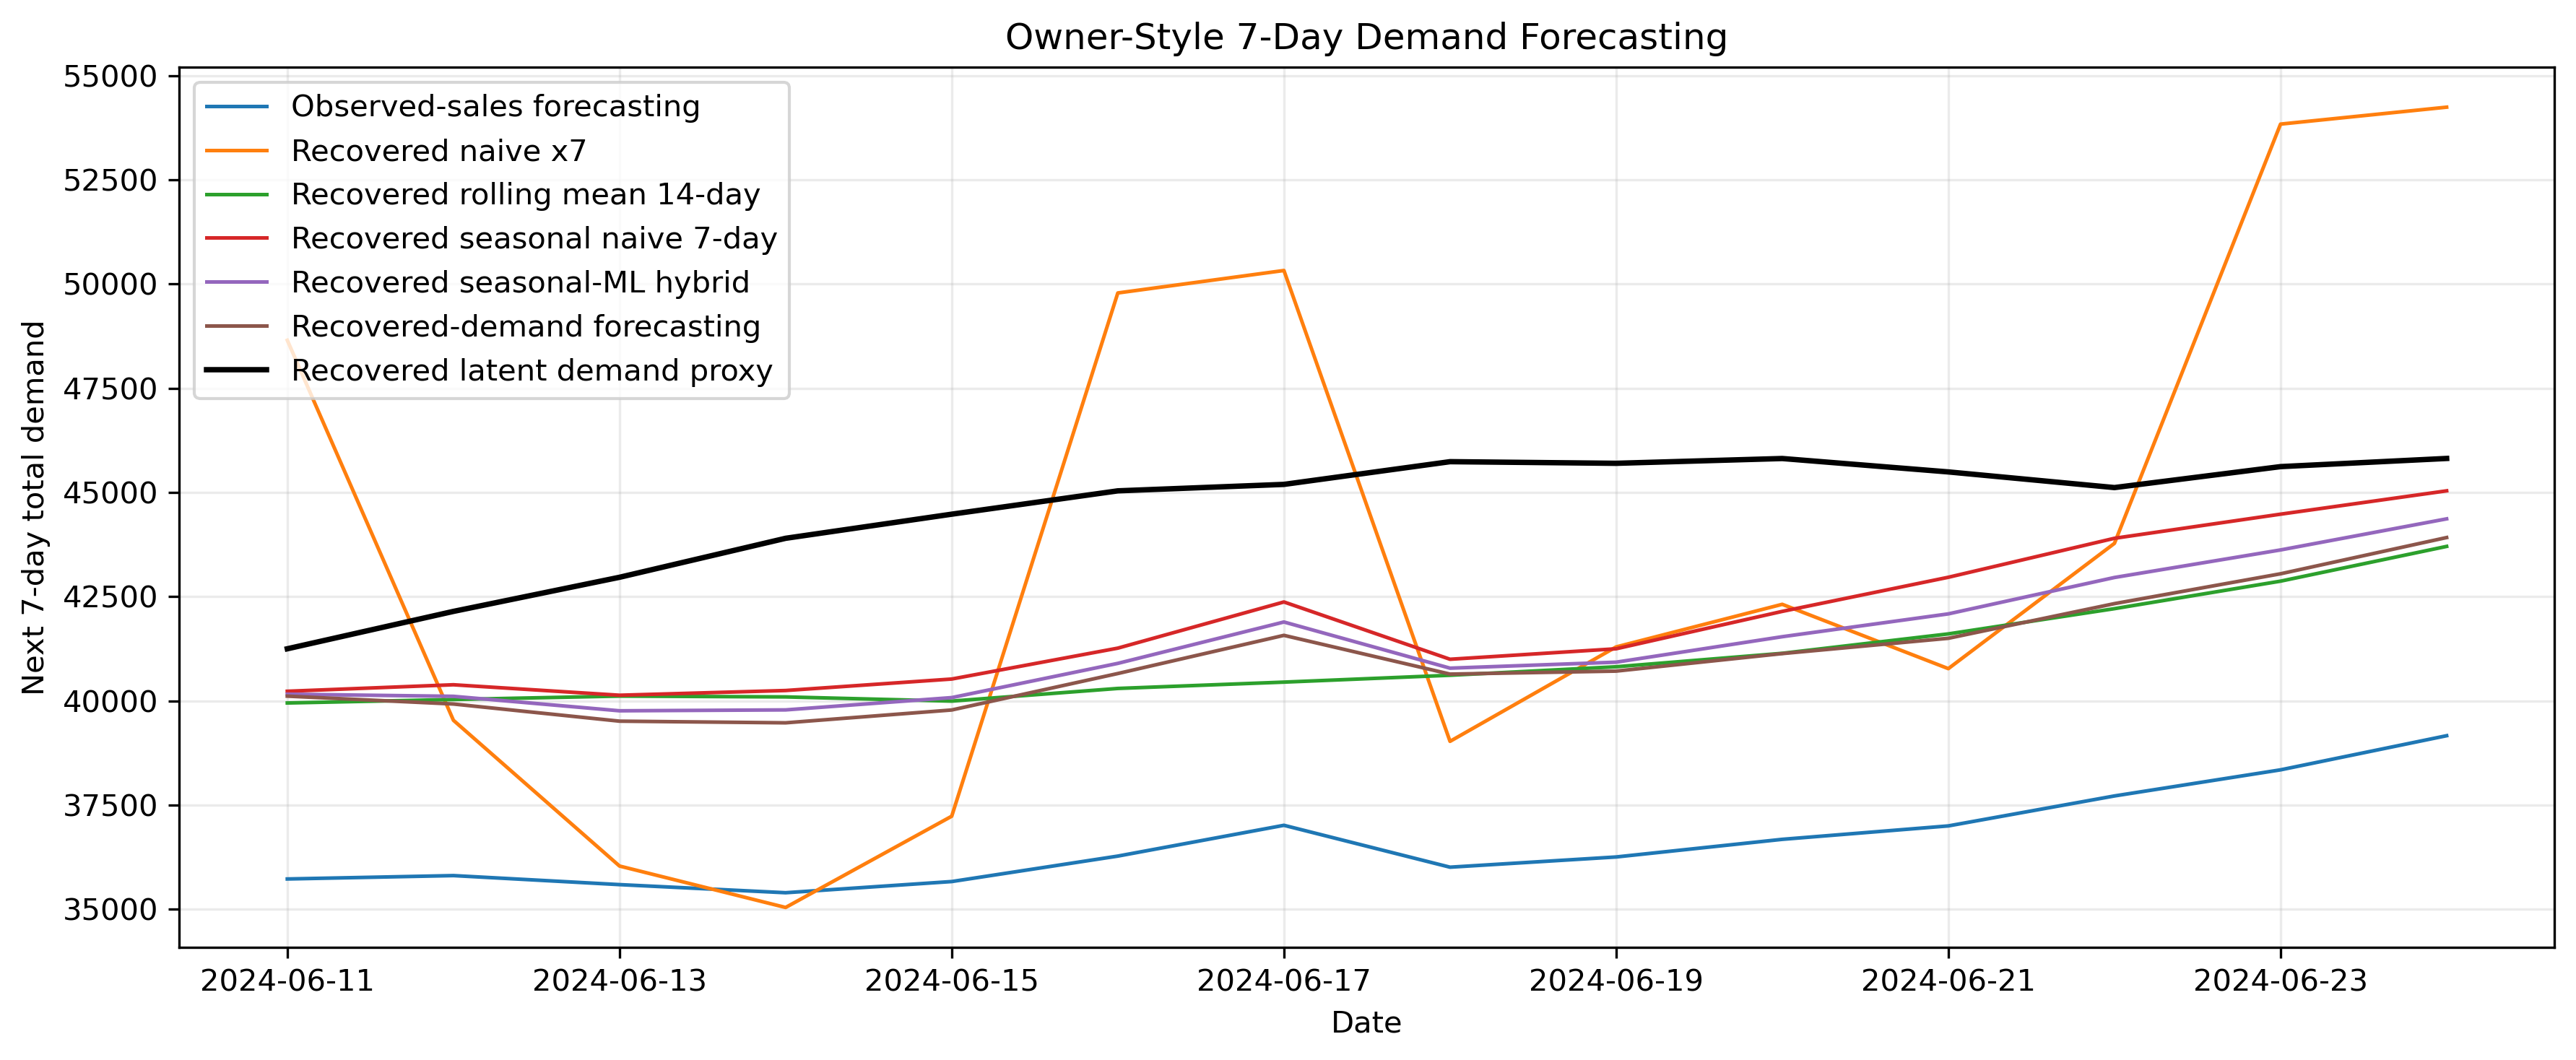
\includegraphics[width=\linewidth]{owner_two_stage_forecast_comparison.png}
        \end{column}
    \end{columns}
\end{frame}

\begin{frame}{Diagnostics và diễn giải}
    \begin{columns}[T]
        \begin{column}{0.50\linewidth}
            \begin{itemize}
                \item Rolling 7-day targets bị overlap mạnh.
                \item Model diagnostics: Recovered seasonal-ML hybrid.
                \item Ljung--Box p-value = 0.0311, còn tự tương quan nhẹ.
                \item Non-overlap check: p-value = 0.1573, không bác bỏ tự tương quan.
                \item Nhưng non-overlap chỉ có 2 điểm aggregate, nên chỉ là kiểm tra phụ.
            \end{itemize}
        \end{column}
        \begin{column}{0.48\linewidth}
            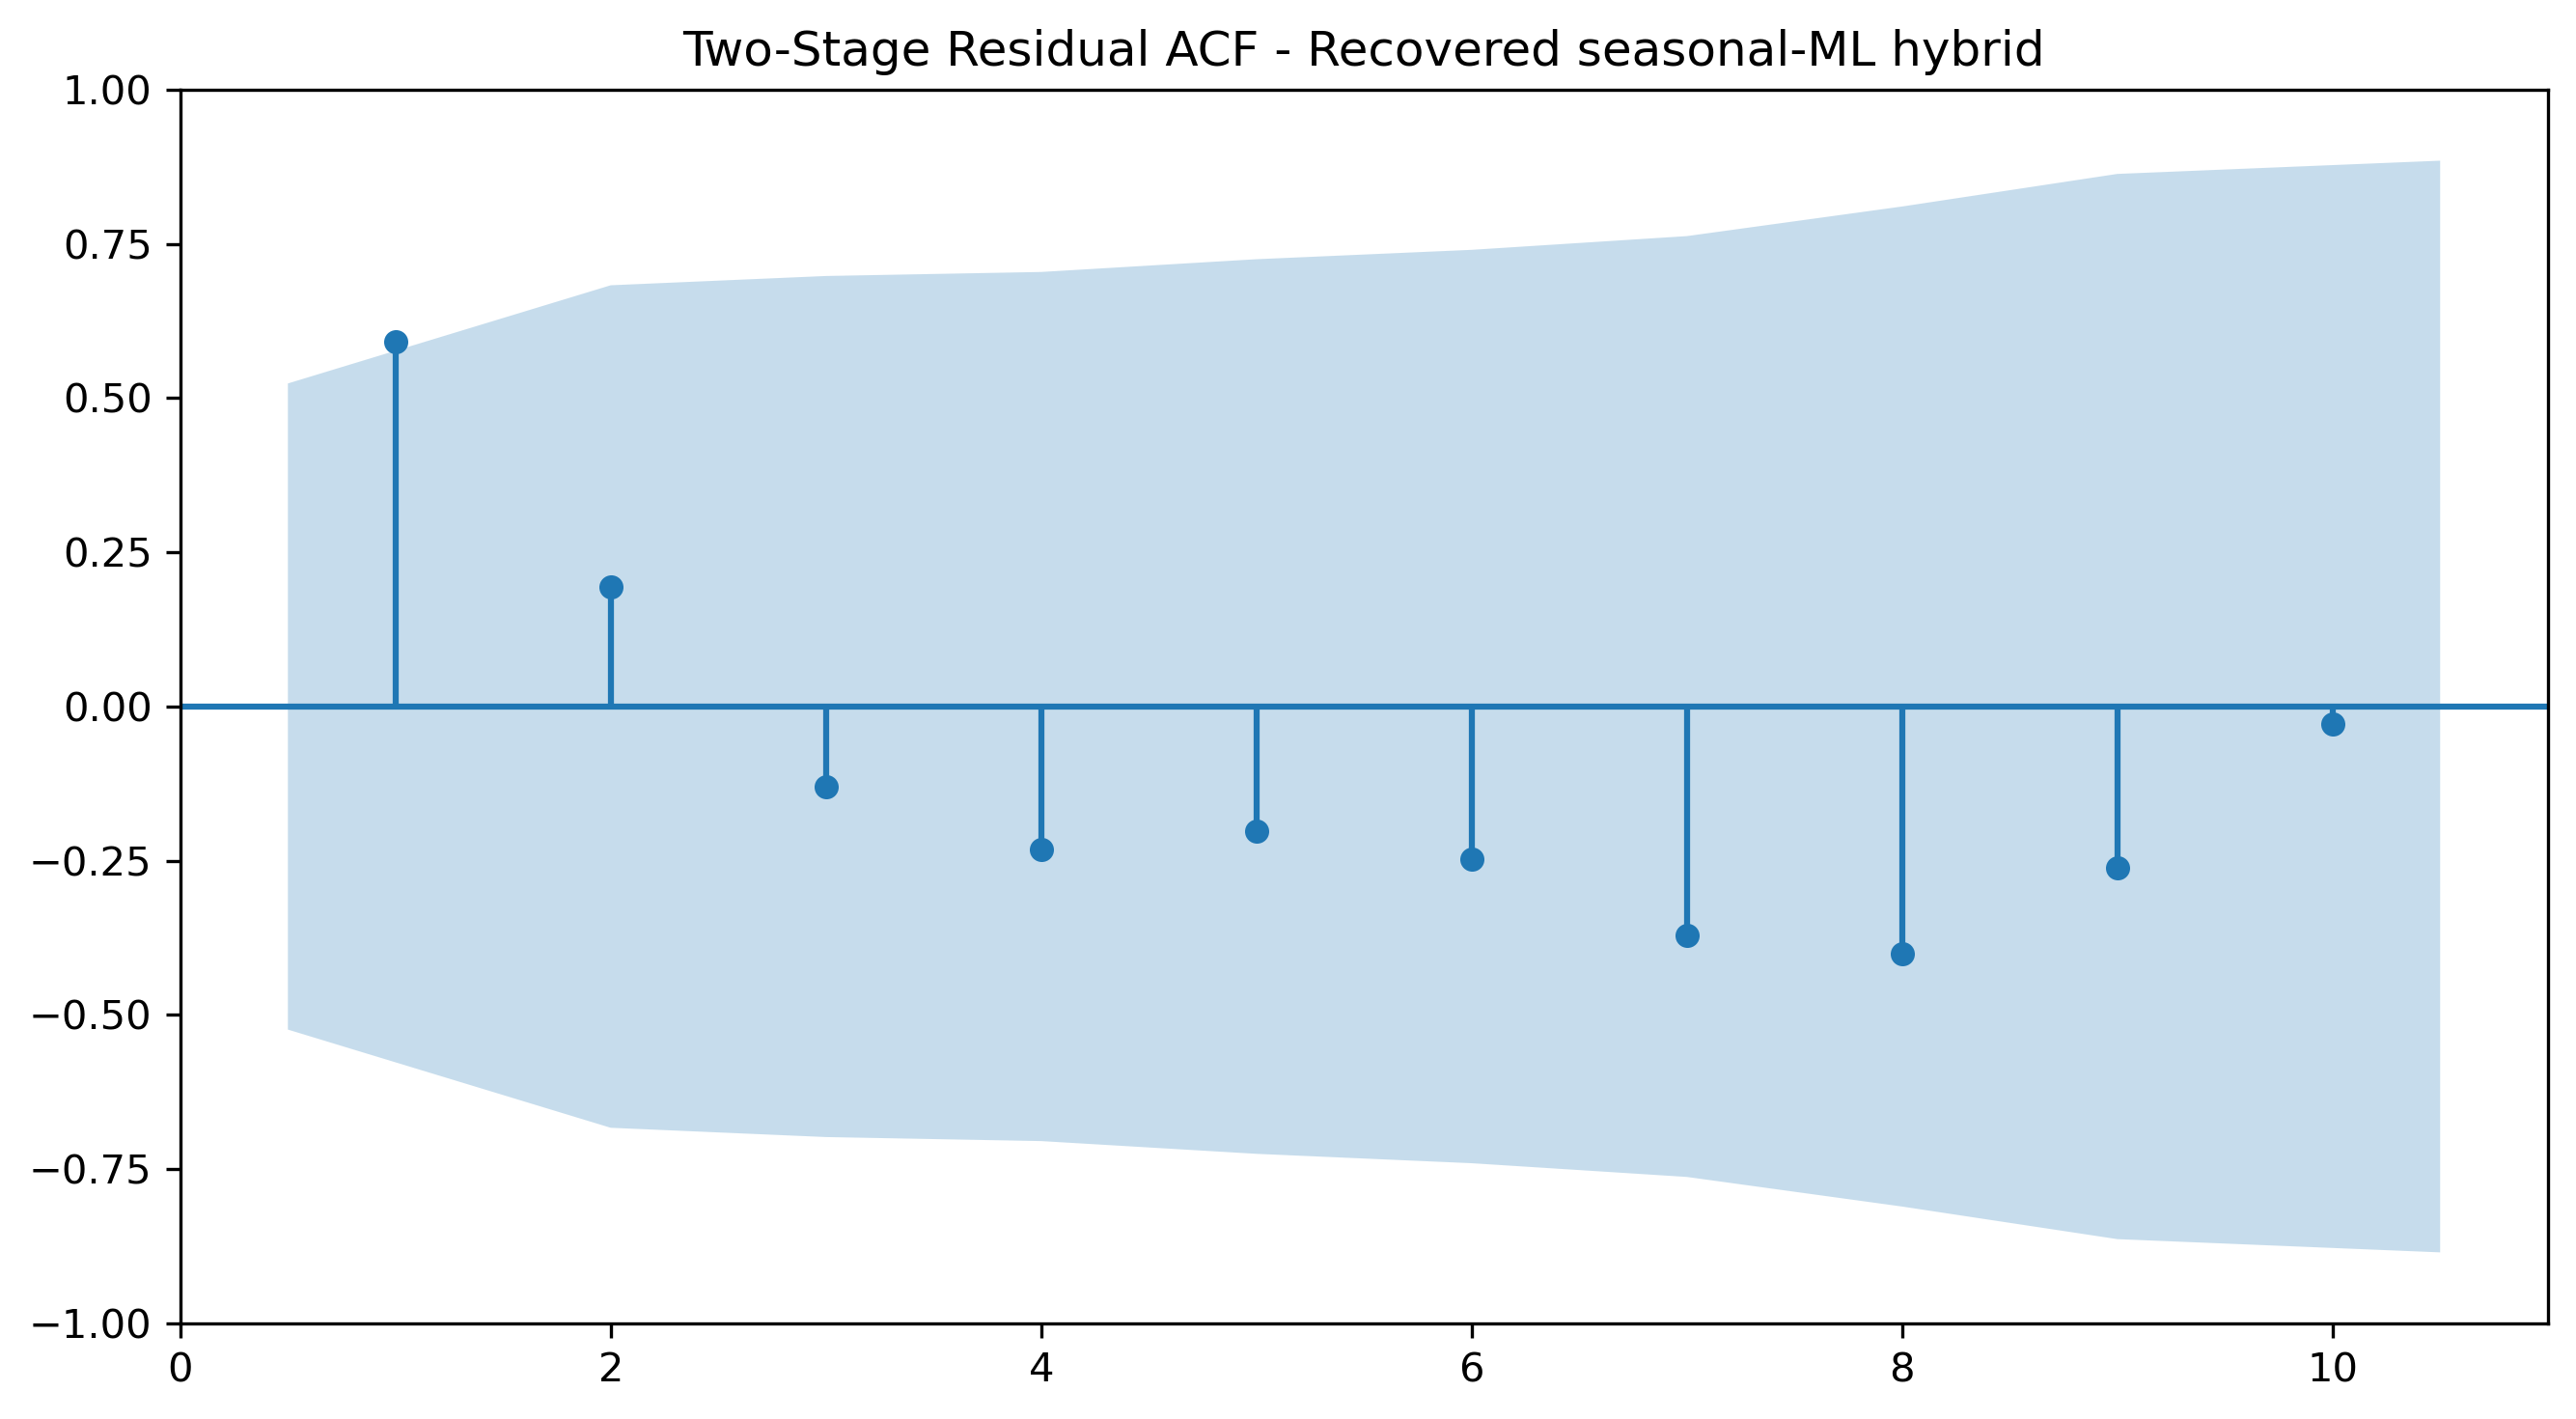
\includegraphics[width=\linewidth]{owner_two_stage_residual_acf.png}
        \end{column}
    \end{columns}
\end{frame}

\begin{frame}{Thông điệp bảo vệ}
    \begin{enumerate}
        \item Framing đúng hơn: forecast demand, không chỉ forecast sales bị giới hạn bởi tồn kho.
        \item Recovery hourly trước, forecast daily sau: phù hợp với bản chất stockout theo giờ và mục tiêu dự báo vận hành.
        \item Imputation có kiểm soát: calibration + cap + sensitivity, lift cuối 10.68\%.
        \item Two-stage có lợi: WAPE giảm từ 24.42\% xuống 19.67\%.
        \item Hạn chế được nói rõ: recovered demand là proxy, residual còn nhiễu, deep imputation có thể là hướng mở rộng.
    \end{enumerate}
\end{frame}

\begin{frame}{Kết luận}
    \begin{block}{Kết luận chính}
    Với dữ liệu bán lẻ có stockout, forecast trực tiếp observed sales dễ học sai nhu cầu. Pipeline two-stage giúp tách bài toán thành recovery demand bị censor và forecast trên demand đã hiệu chỉnh.
    \end{block}
    \vspace{0.2cm}
    \begin{itemize}
        \item Kết quả không chỉ tốt hơn về metric mà còn tốt hơn về lập luận.
        \item WAPE 19.67\% là mức chấp nhận được cho multi-series retail thưa, có stockout.
        \item Điểm mạnh của đồ án là quy trình tránh leakage và kiểm tra imputation rõ ràng.
    \end{itemize}
\end{frame}

\end{document}
